\documentclass[oneside]{article}

% Package necessari
\usepackage[a4paper,top=2cm,bottom=2cm,left=1.5cm,right=1.5cm]{geometry}
\usepackage[utf8]{inputenc}
\usepackage[italian]{babel}
\usepackage[T1]{fontenc}
\usepackage{amsmath}
\usepackage{amssymb}
\usepackage{graphicx}
\usepackage[table, dvipsnames]{xcolor}
\usepackage{listings}
\usepackage{hyperref}
\usepackage{enumitem}
\usepackage{fancyhdr}
\usepackage{cancel}
\usepackage[ruled,vlined,linesnumbered]{algorithm2e}
\usepackage[noend]{algpseudocode}
\usepackage[font={small,sl}]{caption}
\usepackage[font={small,sl}]{subcaption}
\usepackage{tocbibind}
\usepackage{accents}
\usepackage[section]{placeins}
\usepackage{multicol}
\usepackage{mathtools}
\usepackage{dsfont}
\usepackage{color}
\usepackage{titlesec}

\makeatletter
\AtBeginDocument{%
  \expandafter\renewcommand\expandafter\subsection\expandafter{%
    \expandafter\@fb@secFB\subsection
  }%
}
\makeatother

% Colori per i listing
\definecolor{code_red}{rgb}{0.6,0,0} % strings
\definecolor{code_green}{rgb}{0.25,0.5,0.35} % comments
\definecolor{code_purple}{rgb}{0.5,0,0.35} % keywords
\definecolor{code_background}{rgb}{0.95,0.95,0.92} % background
\definecolor{verify_blue}{HTML}{12ACF2}
\definecolor{verify_red}{HTML}{F2122C}
\definecolor{verify_yellow}{HTML}{FFBB00}

% Stile del codice standard (C)
\lstset{
	language=C, 
	backgroundcolor=\color{code_background},
	frame=single,
	basicstyle=\ttfamily\small,
	keywordstyle=\color{code_purple}\bfseries\small,
	stringstyle=\color{code_red}\small,
	commentstyle=\color{code_green}\small,
	numbers=left,
	numberstyle=\small\color{gray},
	numbersep=5pt,
	tabsize=4,
	showtabs=false,
	showspaces=false,
	showstringspaces=false,
	escapechar=|, 
	captionpos=b,
	breaklines=true,
}

% Aggiunto paragraph come subsubsubsection
\setcounter{secnumdepth}{3}
\titleformat{\paragraph}
{\normalfont\normalsize\bfseries}{\theparagraph}{1em}{}
\titlespacing*{\paragraph}
{0pt}{3.25ex plus 1ex minus .2ex}{1.5ex plus .2ex}

% Impostazione delle lunghezze di alcuni elementi del documento
\setlength{\parskip}{1em}
\setlength{\parindent}{0em}
\setlength{\arrayrulewidth}{0.1em}

% Informazioni per la title page
\title{Progetto di Sistemi Operativi Avanzati}

\date{A.A. 2021/2022}

\author{A. Chillotti\thanks{\texttt{\href{mailto:alessandro.chillotti@outlook.it}{alessandro.chillotti@outlook.it}}}}

% Impostazione del package hyperref
\hypersetup{
    colorlinks=true,
    linktocpage=true,
    linkcolor=blue,
    urlcolor=blue,
    pdftitle={Advanced Operating Systems and System Security},
    pdfauthor={A. Chillotti},
}
 
% Stile del codice standard (C)
\lstset{
	language=C, 
	backgroundcolor=\color{code_background},
	frame=single,
	basicstyle=\ttfamily\small,
	keywordstyle=\color{code_purple}\bfseries\small,
	stringstyle=\color{code_red}\small,
	commentstyle=\color{code_green}\small,
	numbers=left,
	numberstyle=\small\color{gray},
	numbersep=5pt,
	tabsize=4,
	showtabs=false,
	showspaces=false,
	showstringspaces=false,
	escapechar=|, 
	captionpos=b,
	breaklines=true,
}

\pagestyle{fancy}
\fancyhf{}
\lhead{\small A.Chillotti}
\rhead{\small Advanced Operating Systems and System Security}
\cfoot{\thepage}
%\cfoot{Pagina \thepage}
\SetNlSty{bfseries}{\color{black}}{}

% Spaziatura tabelle
\renewcommand{\arraystretch}{1.5}

\graphicspath{ {./figs/} }
% Definizione del colore delle tabelle
\newcommand{\tablecolors}[1][2]{\rowcolors{#1}{yellow!50}{yellow!25}}

% Definizione dello stile da usare per la P di probabilità (grassetto in math-mode)
\newcommand{\pr}{\mathbf{P}}

% Forzatura del displaystyle in math-mode
\everymath\expandafter{\the\everymath\displaystyle}

%\newcommand{\scaption}[1]{\small{\caption{#1}}}
\renewcommand{\lstlistingname}{Snippet}

% Definizione di comandi per operatori matematici
\newcommand{\xor}{\oplus}

% Definizione osservazione
\newcommand{\obs}{\underline{Osservazione}}

% Definizione di \texttt{•} per matematica
\newcommand{\matht}[1]{\text{\texttt{#1}}}

% Definizione di domande e risposta
\newcommand{\question}[2]{
\textit{#1}\\
#2
}

\begin{document}
\maketitle

\section{Traccia del progetto (traduzione)}
Questa specifica è legata ad un driver Linux che implementa flussi di dati a priorità bassa e alta. Attraverso una sessione aperta al devide file, un thread può leggere/scrivere segmenti dati. La consegna dei dati segue una policy First-in-First-out lungo ciascuno dei due diversi flussi di dati (bassa e alta priorità). Dopo le operazioni di lettura, i dati devono scomparire dal flusso. Inoltre, il flusso dati di alta priorità deve offrire operazioni di scrittura sincrone, mentre il flusso dati di bassa priorità deve offrire una esecuzione asincrona (basata su delayed work) delle operazioni di scrittura, pur mantenendo l'interfaccia in grado di notificare in modo sincrono l'esito. Le operazioni di lettura sono tutte eseguite sincronamente. Il device driver supporta 128 device corrispondenti alla stessa quantità di minor number. Il device driver deve implementare il supporto per il servizio \texttt{ioctl(..)} in modo tale da gestire la sessione di I/O come segue:
\begin{itemize}
\item setup del livello di priorità (alto o basso) per le operazioni;
\item operazioni di lettura e scrittura bloccanti vs operazioni di lettura e scrittura non bloccanti;
\item setup del timeout che reluga il risveglio delle operazioni bloccanti.
\end{itemize}
Alcuni parametri e funzioni del modulo Linux dovrebbero essere in grado di abilitare o disabilitare il file del dispositivo, in termini di specifico minor number. Se è disabilitato, un tentativo di apertura della sessione deve fallire (ma le sessioni già aperte devono essere ancora gestire). Ulteriori parametri esposti via VFS devono fornire un'immagine dello stato corrente del device in accordo alle seguenti informazioni:
\begin{itemize}
\item abilitiato o disabilitato;
\item numero di byte correntemente presente nei due flussi (alta e bassa priorità);
\item numero di thread correntemente in attesa di dati lungo i due flussi (alta e bassa priorità).
\end{itemize}

\section{Relazione del progetto svolto}
\subsection{Rappresentazione dei multi-flow device file}
La rappresentazione dei multi-flow device file è definita dalla struttura \texttt{object\_t} che contiene:
\begin{itemize}
\item un puntatore ad una workqueue, ovvero \texttt{struct workqueue\_struct *workqueue}. Il puntatore alla workqueue è stato inserito all'interno della struttura che rappresenta il multi-flow device file perché è utile solo nel caso in cui si sta lavorando a \texttt{LOW PRIORITY}.
\item due puntatori ad un buffer, ovvero \texttt{dynamic\_buffer\_t *buffer}.
\end{itemize}

\subsection{Rappresentazione del buffer}
La rappresentazione del buffer è definita dalla struttura \texttt{dynamic\_buffer} che contiene:
\begin{itemize}
\item un puntatore \texttt{head} di tipo \texttt{list\_head};
\item un mutex che permette di sincronizzare le operazioni relative al buffer;
\item una waitqueue.
\end{itemize}
Quindi, l'idea è che il multi-flow device driver si appoggi su un ulteriore oggetto, il \texttt{dynamic buffer}, che ci occupa di scrivere e leggere segmenti dati.


Si può notare come siano presenti \texttt{256} waitqueue, ovvero una per ogni buffer. Questa scelta è stata fatta perché il lavoro svolto su un buffer è sicuramente indipendente dal lavoro compiuto su un altro. Inoltre, nella funzione di inizializzazione del modulo vengono create delle singlethread workqueue. In questo modo il deferred work viene processato lungo un unico kworker deamon ed esso riporta le operazioni di scrittura sul buffer di bassa priorità nel medesimo ordine con cui sono state schedulate, senza dover implementare meccanismi di ordinamento e sincronizzazione.

\subsection{Parametri del modulo}
Sono stati definiti dei parametri del modulo ed essi sono stati utilizzati all'interno del driver come variabili operative. In particolare sono stati definiti i seguenti parametri:
\begin{itemize}
\item \texttt{enabled}: un vettore di \texttt{128} elementi di tipo \texttt{bool}, ove ogni elemento \texttt{i} indica se il multi-flow device relativo al minor number \texttt{i} è attivo o meno;
\item \texttt{byte\_in\_buffer}: un vettore di \texttt{256} elementi di tipo \texttt{long}, ove ogni elemento riporta il numero di byte presenti all'interno del buffer relativo ad uno specifico minor number, in particolare:
\begin{itemize}
\item i primi \texttt{128} elementi sono relativi al buffer di bassa priorità del multi-flow device con minor number \texttt{i};
\item i secondi \texttt{128} elementi sono relativi al buffer di alta priorità del multi-flow device con minor number $(\mathtt{i-128})$.
\end{itemize}
\item \texttt{thread\_in\_wait}: un vettore di \texttt{256} elementi di tipo \texttt{long}, ove ogni elemento riporta il numero di byte presenti all'interno del buffer relativo ad uno specifico minor number, secondo la medesima regola di \texttt{byte\_in\_buffer}.
\end{itemize}

La scelta di creare un vettore di \texttt{256} elementi anziché \texttt{128} è stata fatta perché ha permesso la realizzazione di un codice migliore dal punto di vista della leggibilità. Questo perché, indipendentemente dalla priorità, prima di andare ad effettuare una scrittura o una lettura si effettua un controllo sul contenuto del buffer (i.e. spazio libero in caso di scrittura, byte nel buffer in caso di lettura). Infatti, nel caso in cui si fossero creati due vettori da \texttt{128} elementi si sarebbero dovuti differenziare i casi. A tal proposito è stata realizzata la seguente macro:
\begin{lstlisting}
#define get_byte_in_buffer_index(priority, minor)	\
        ((priority * MINOR_NUMBER) + minor)
\end{lstlisting}

Inoltre, si può notare come in questo modo non venga effettuato nessun check, ma una semplice operazione matematica.

Per lavorare con i parametri del modulo sono stati sviluppati degli script bash:
\begin{itemize}
\item lo script \texttt{enable\_set} consente di settare l'abilitazione del multi-flow device per un certo minor;
\item lo script \texttt{enable\_query} consente di sapere se il multi-flow device è abilitato o meno per un certo minor;
\item lo script \texttt{byte\_query} consente di sapere, data la priorità ed il minor, il numero di byte presenti nel buffer associato;
\item lo script \texttt{thread\_query} consente di sapere, data la priorità ed il minor, il numero di thread in attesa sul flusso associato.
\end{itemize}
\subsection{Operazioni sui multi-flow device file}
Nelle seguenti sottosezioni sono descritte le funzioni che compongono il driver.

\subsection{Operazione d'apertura}
La funzione \texttt{dev\_open} consente l'apertura di una sessione per poter lavorare con un determinato multi-flow device file. In questa funzione vengono effettuate le seguenti operazioni:
\begin{enumerate}
\item Viene controllato che il \texttt{minor} inserito sia effettivamente minore o uguale rispetto al \texttt{minor} massimo gestibile dal driver.
\item Viene controllata la componente del vettore \texttt{enabled}, ovvero si controlla che il \texttt{minor} verso il quale si vuole aprire una sessione abbia il multi-flow device controller effettivamente abilitato.
\item Nel caso in cui entrambi i controlli abbiano avuto esito positivo, si prepara la struttura ad-hoc \texttt{session\_t} settando di default i seguenti parametri:
\begin{itemize}
\item come priorità viene inserita \texttt{HIGH PRIORITY};
\item viene settata come sessione bloccante, ovvero viene settato il campo \texttt{flags}\footnote{In caso di operazione non bloccante, si avrà settato questo campo come \texttt{GFP\_ATOMIC}.} a \texttt{GFP\_KERNEL};
\item viene settato il timeout a \texttt{MAX\_SECONDS}.
\end{itemize}
\item Viene collegata questa istanza \texttt{session\_t} alla componente \texttt{file->private\_data}.
\end{enumerate}

È importante precisare che la macro \texttt{MAX\_SECONDS} è stata settata al valore \texttt{17179869} perché, nel momento in cui si inserisce il valore da attendere all'interno della \texttt{wait\_event\_interruptible\_exclusive\_timeout}\footnote{Questa macro è stata sviluppata durante la stesura del progetto, più avanti verrà analizzata e motivata.}, bisogna inserire il numero di secondi moltiplicato per la costante \texttt{HZ}, ove in questo caso è pari a \texttt{250}. Il ragionamento effettuato è il seguente:
\begin{equation*}
2^{32} = 4294967296 \rightarrow \frac{4294967296}{250} = 17179869.184 \rightarrow \mathtt{MAX\_SECONDS} = 17179869
\end{equation*}
In questo modo si evita l'overflow nel momento in cui si effettua l'operazione di settaggio del timeout.

\subsection{Operazione di rilascio}
La funzione \texttt{dev\_release} consente il rilascio della sessione per poter lavorare con un determinato multi-flow device file. In questa funzione viene effettuata la \texttt{kfree} di ciò presente all'indirizzo inserito in \texttt{file->private\_data}, quindi dell'indirizzo della \texttt{session\_t} preparata all'interno dell'operazione d'apertura.

\subsection{Operazione di scrittura}
La funzione \texttt{dev\_write} consente la scrittura del contenuto di un buffer di livello user all'interno del buffer di livello kernel. In questa funzione avvengono le seguenti operazioni:
\begin{itemize}
\item Una prima fase di allocazione di aree di memoria:
\begin{enumerate}
\item Viene allocato un buffer temporaneo di livello kernel e subito dopo viene effettuata la \texttt{copy\_from\_user}.

Questo viene fatto prima di prendere il lock perché, nel caso in cui l'utente avesse dato un'area di memoria non materializzata, si sarebbe dovuto attendere il gestore di page fault e avrebbe causato problemi di prestazioni.
\item Viene allocata l'area di memoria per il \texttt{data\_segment} corrente, ovvero l'oggetto da inserire all'interno del \texttt{dynamic buffer}.
\item Nel caso in cui la priorità sia bassa, viene allocata l'area di memoria per poter inserire deferred work.
\end{enumerate}
Come si può notare, questa fase viene effettuata prima di provare ad acquisire il lock in modo tale che non ci possano essere problemi di allocazione nel momento in cui si possiede il lock.
\item Una seconda fase in cui si cerca di acquisire il lock e ci sono due casi:
\begin{itemize}
\item Nel caso in cui le operazioni sono bloccanti:
\begin{enumerate}
\item Viene incrementata la variabile che tiene conto dei thread in attesa.
\item Si va nella \texttt{wait\_event\_interruptible\_exclusive\_timeout} con la condizione che è dettata dalla macro \texttt{lock\_and\_awake}.

La macro \texttt{lock\_and\_awake} è la seguente:
\begin{lstlisting}[caption={Macro \texttt{lock\_and\_awake}},label={macrolock}]
#define lock_and_awake(condition, mutex)		\
({												\
        int __ret = 0;							\
        if (mutex_trylock(mutex)) {             \
                if (condition)                  \
                        __ret = 1;              \
                else                            \
                        mutex_unlock(mutex);    \
        }                                       \
        __ret;                                  \
})
\end{lstlisting}
Questa macro ritorna \texttt{0} se il thread non è riuscito a prendere il lock o, nel caso in cui ci fosse riuscito, non abbia soddisfatto la condizione. In questo caso la condizione riguarda il fatto che nel buffer ci sia spazio o sia interamente occupato.

Da notare che viene chiamata la \texttt{wait\_event\_interruptible\_exclusive\_timeout}\footnote{Le macro chiamate da essa, ovvero la \texttt{\_\_wait\_event} e la \texttt{\_\_wait\_cond\_timeout}, sono definite a parire dal kernel 3.13, infatti all'interno del codice è presente il check sulla versione e, se inferiore a 3.13, viene chiamata semplicemente la \texttt{wait\_event\_interruptible\_timeout}.} che non è definita nel kernel Linux, ma questo è stato fatto perché serviva una soluzione che potesse risolvere i seguenti problemi:
\begin{itemize}
\item Utilizzando \texttt{wait\_event\_interruptible\_timeout} internamente i thread si sarebbero svegliati tutti e poi avrebbero controllato la condizione, ma solamente uno sarebbe riuscito ad uscire dalla wait. Questo avrebbe comportato uno spreco di cicli di CPU.
\item Utilizzando \texttt{wait\_event\_interruptible\_exclusive} si sarebbe dovuto implementare un meccanismo separato di gestione del timeout andando ad aggiungere complessità al prodotto software.
\end{itemize}
Si è pensato che in questo modo la complessità del prodotto software non sia stata alterata e che risulti anche abbastanza elegante per la risoluzione del primo problema. Infatti, è stata modificata la funzione \texttt{\_\_wait\_event\_interruptible\_timeout}, in particolare:
\begin{figure}[ht!]
\centering
\frame{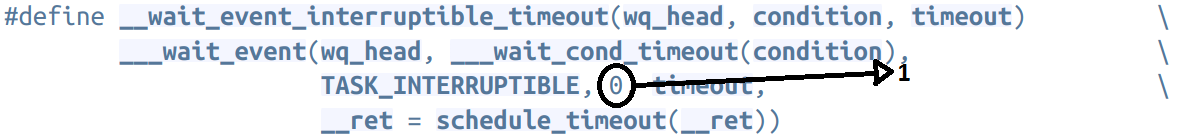
\includegraphics[width=0.6\textwidth]{img/fig-wait}}
\caption{Modifica della \texttt{wait\_event\_interruptible\_timeout}}
\label{img:fig-wait}
\end{figure}

In relazione alla documentazione (\href{https://www.makelinux.net/ldd3/chp-6-sect-2.shtml}{link}, \textit{6.2.5.3 Exclusive waits}), si può notare che gli sviluppatori del kernel hanno aggiunto un'opzione di "attesa esclusiva" al kernel. Un'attesa esclusiva si comporta in modo molto simile a un normale sonno, con due importanti differenze:
\begin{itemize}
\item Quando una voce della coda di attesa ha il flag \texttt{WQ\_FLAG\_EXCLUSIVE} impostato, viene aggiunta alla fine della coda di attesa. Le voci senza quel flag vengono, invece, aggiunte all'inizio.
\item Quando \texttt{wake\_up} viene chiamato su una coda di attesa, si interrompe dopo aver riattivato il primo processo con il flag \texttt{WQ\_FLAG\_EXCLUSIVE} impostato.
\end{itemize}
In figura \ref{img:fig-wait} si può notare come ogni thread venga mandato a dormire con il flag \texttt{WQ\_FLAG\_EXCLUSIVE} impostato, ma inoltre rimane valido lo \texttt{schedule\_timeout}.
\item Quando il thread riprende l'esecuzione decrementa la variabile precedentemente incrementata e, se si è svegliato perché \texttt{lock\_and\_awake} ha ritornato \texttt{1}, allora prosegue l'esecuzione nella terza fase.
\end{enumerate}
\newpage
\item Nel caso in cui le operazioni non sono bloccanti:
\begin{enumerate}
\item Si prova a prendere il lock ed in caso negativo si rilasciano le aree allocate e si ritorna \texttt{EBUSY}.
\item Se il lock è stato acquisito si controlla se il buffer è vuoto, in tal caso si rilasciano le aree allocate, il lock e si chiama la \texttt{wake\_up\_interruptible}.
\end{enumerate}
\end{itemize}
\item La terza fase riguarda la fase di scrittura del segmento dati e, dopo aver fatto un controllo sulla dimensione dei dati da scrivere e fatto la \texttt{init\_data\_segment}, ci sono due casi:
\begin{itemize}
\item Nel caso di \texttt{HIGH PRIORITY}:
\begin{enumerate}
\item Viene invocata la \texttt{write\_dynamic\_buffer} sull'oggetto \texttt{dynamic\_buffer}, quindi viene effettuata la scrittura.
\item Viene incrementato il numero di byte nel buffer e viene invocata la \texttt{wake\_up\_interruptible}.
\end{enumerate}
\item Nel caso di \texttt{LOW PRIORITY}:
\begin{enumerate}
\item Si chiama la \texttt{try\_module\_get}.
\item Si collega solamente\footnote{Questo è un vantaggio in termini di performance perché all'interno della sezione critica si ha bisogno solamente di collegare il contenuto da scrivere alla struttura del deferred work.} il contenuto da scrivere al deferred work.
\item Si chiama \texttt{\_\_INIT\_WORK}.
\item Si incrementano i byte prenotati.
\item Si accoda il lavoro nella workqueue.
\end{enumerate}
\end{itemize}
\item L'ultima fase si occupa solo del rilascio del lock acquisito e ritorna i byte scritti.
\end{itemize}

\subsubsection{Scrittura differita}
È stata creata una funzione ad-hoc che si occupa della scrittura differita ed essa effettua le seguenti operazioni:
\begin{enumerate}
\item Si effettua la \texttt{mutex\_lock}. In questo caso si è bloccanti perché una volta che i byte sono stati prenotati devo essere assolutamente scritti.
\item Si chiama la \texttt{write\_dynamic\_buffer}.
\item Si decrementa il numero di byte prenotati e si incrementa il numero di byte nel buffer.
\item Si rilascia il lock e si rilascia l'area di memoria della \texttt{work\_struct}.
\item Si chiama \texttt{wake\_up\_interruptible} e \texttt{module\_put}.
\end{enumerate}

\subsection{Operazione di lettura}
La funzione \texttt{dev\_read} consente la lettura del contenuto del buffer di livello kernel e lo spostamento del contenuto letto all'interno del buffer di livello user. In questa funzione avvengono le seguenti operazioni:
\begin{enumerate}
\item Il primo controllo effettuato riguarda il numero di byte che l'utente vuole leggere, infatti se il numero di byte è pari a \texttt{0} si ritorna immediatamente \texttt{0} in modo tale da non consumare inutilmente cicli di CPU.
\item Viene allocata l'area di memoria per un buffer temporaneo.
\item Anche qui ci sono due strade:
\begin{itemize}
\item Nel caso bloccante, si segue lo stesso approccio della funzione \texttt{dev\_write}, ma la condizione con cui si va a dormire riguarda ovviamente la presenza di byte da leggere.
\item Anche il caso non bloccante è simile all'approccio della funzione \texttt{dev\_read}.
\end{itemize}
\item Dopo un controllo sulla dimensione dei byte da leggere, viene invocata la \texttt{read\_dynamic\_buffer}.
\item Viene decrementato il numero di byte nel buffer.
\item Si fa l'\texttt{unlock} e si effettua la \texttt{copy\_to\_user}.
\item Si ritorna il numero di byte consegnati a livello di user.
\end{enumerate}

\subsection{Operazione \texttt{ioctl}}
La funzione che risponde alle richieste di gestione di un multi-flow device file è la funzione \texttt{dev\_open}. Sono stati definiti dei codici che permettono di identificare i comandi:
\begin{itemize}
\item il codice \texttt{TO\_HIGH\_PRIORITY} permette di settare il livello di priorità come alto;
\item il codice \texttt{TO\_LOW\_PRIORITY} permette di settare il livello di priorità come basso;
\item il codice \texttt{BLOCK} permette di settare le operazioni come bloccanti;
\item il codice \texttt{UNBLOCK} permette di settare le operazioni come non bloccanti;
\item il codice \texttt{TIMEOUT} permette di settare un timeout, infatti viene chiesto un argomento da passare alla funzione di \texttt{ioctl}.
\end{itemize}

Inoltre, è stata definita una piccola libreria che permette di rendere trasaparente l'invio di richieste I/O control, ovvero senza dover conoscere i codici. La libreria consiste in delle macro che espandono in invocazione di \texttt{ioctl} con il relativo codice ed eventualmente con l'apposito argomento.

\subsection{Ulteriore osservazione}
All'interno del codice è stata utilizzato il costrutto \texttt{unlikely} nei check degli errori riguardanti l'allocazione di memoria. Se ci fosse stato a disposizione un operation profile sarebbe stato interessante andare ad usare \texttt{likely/unlikely} per favorire la predizione dei salti, ad esempio se si fosse saputo che il 90\% dei thread fosse \texttt{HIGH PRIORITY}, si sarebbe potuto mettere \texttt{likely} sul controllo \texttt{priority == HIGH PRIORITY} e \texttt{unlikely} sul duale.

\end{document}
